%%%%%%%%%%%%%%%%%%%%%%%%%%%%%%%%%%%%%%%%%%%%%%%%%%%%%%%%%%%%%%%%%%%%%%%%
\section{Assignment}
\subsection{Overview}

\subsection{Results}

Data was downloaded from \url{http://sidc.be/silso/datafiles} and \url{ftp://ftp.ngdc.noaa.gov/STP/GEOMAGNETIC_DATA/INDICES/KP_AP}, year 2003, and the data format was checked.
\subsection{Discussion}




%%%%%%%%%%%%%%%%%%%%%%%%%%%%%%%%%%%%%%%%%%%%%%%%%%%%%%%%%%%%%%%%%%%%%%%%
\section{Assignment}
\subsection{Overview}
\subsection{Results}
For the default case, the number density is much lower at higher altitudes than it is for the corrected value, for example: at an altitude of approx. 500km the number density is around $10^{5.05}$, whereas for the latter case the number density at 500km is approx. $10^{5.2}$.
\textbf{insert the images here}
\subsection{Discussion}





%%%%%%%%%%%%%%%%%%%%%%%%%%%%%%%%%%%%%%%%%%%%%%%%%%%%%%%%%%%%%%%%%%%%%%%%
\section{Assignment}
\subsection{Overview}
\subsection{Results}
for 2003
SD:7.1
average sunspot number 99.3

Selecting Day 1

\todo{insert plot here}

The sunspot number parameter has almost no effect at lower altitudes, however at approx. 250km the electron number density starts to vary. The lower the sunspot number the lower the electron number density at each respective altitude above 250km.
\todo{insert plot here km/e-}

2. The electron number density varies on a diurnal basis, but only very minutely. 

3. Comparing Winter and Summer (day 1 and day 181), the electron number density varies on a larger scale.
\subsection{Discussion}



%%%%%%%%%%%%%%%%%%%%%%%%%%%%%%%%%%%%%%%%%%%%%%%%%%%%%%%%%%%%%%%%%%%%%%%%
\section{Assignment}
\subsection{Overview}
\subsection{Results}
Since the given latitude and longitude are located in the auroral region, and 2003 was close to a maximum of the sun's 11-year cycle, the IRI2001 Model is not suitable as this is not magnetically-quite region.
\subsection{Discussion}



%%%%%%%%%%%%%%%%%%%%%%%%%%%%%%%%%%%%%%%%%%%%%%%%%%%%%%%%%%%%%%%%%%%%%%%%
\section{Assignment}
\subsection{Overview}
\subsection{Results}
\todo{todo}
D-Layer below 90

E 90-130

F1-130
\begin{figure}[h]
	\centering
	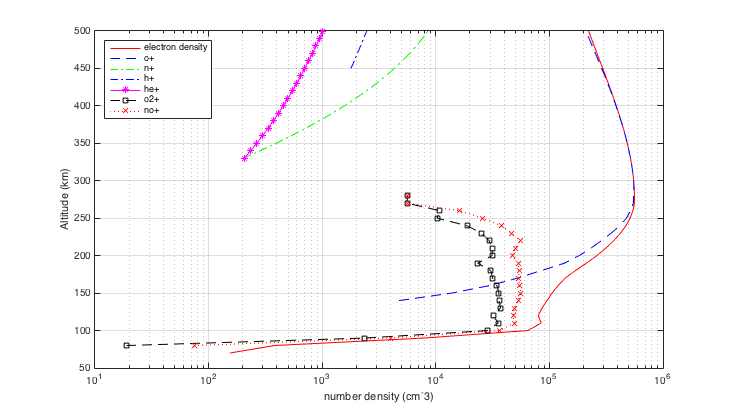
\includegraphics[width=\linewidth]{images/ass5_properties_plot}	
	\caption{bla}
	\label{fig:ass5Plot}
\end{figure}


\subsection{Discussion}

